\chapter{Anforderungen}
\label{cha:Anforderungen}

\section{Benutzerfreundlichkeit aus dem Gesichtspunkt der Systemintegratoren}

\section{Zu unterstützende Plattformen}

Vorgaben WinCC OA, zu 

\subsection{SUSE Linux Enterprise Server}

\subsection{Windows}

\section{Anwendungsfälle}

Use case diagramme + beschreibung etc.

\subsection{Remote-Fehleranalyse und Datenabfrage}

\subsection{Entwicklung kundenspezifischer Anforderungen}

\begin{figure}[h]
	\centering 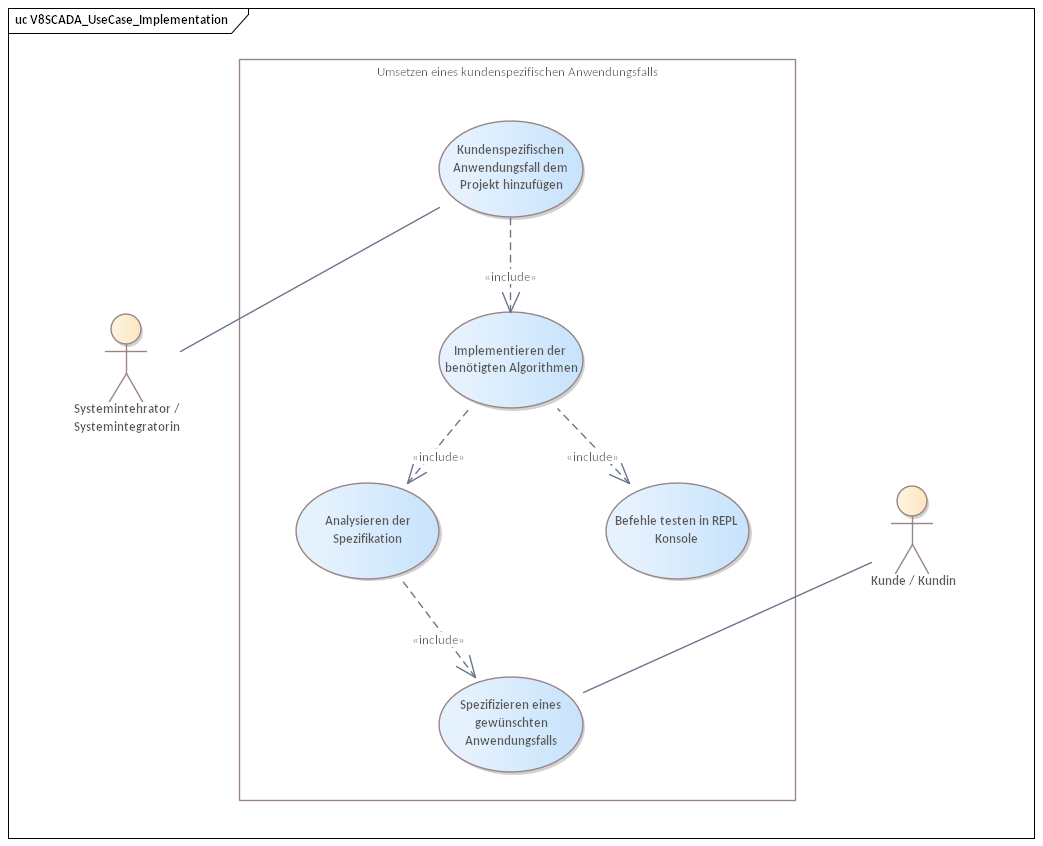
\includegraphics[width=1\textwidth]{UseCase_Implementation}
	\caption{a}
	\label{fig:UseCase_Implementation}
\end{figure}

In dem gezeigten Beispiel \ref{fig:UseCase_Implementation}

\subsection{Skriptgesützte Massenparametrierung}

\begin{figure}[h]
	\centering 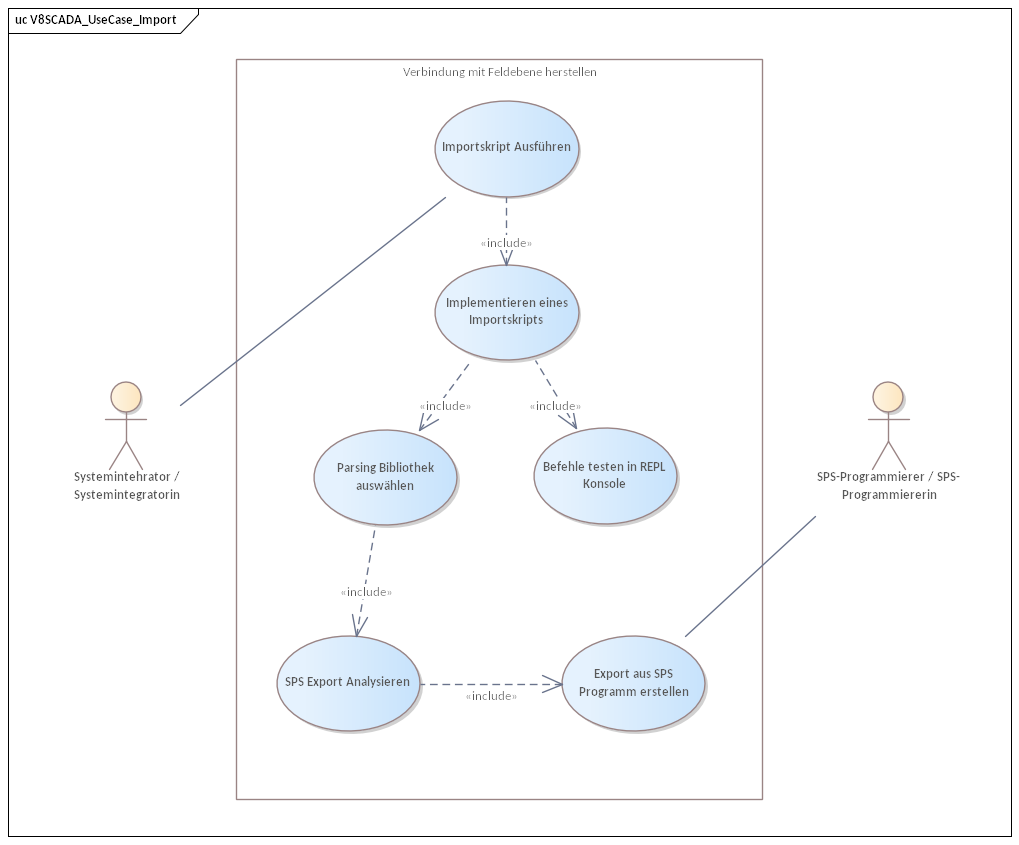
\includegraphics[width=1\textwidth]{UseCase_Import}
	\caption{a}
	\label{fig:UseCase_Import}
\end{figure}

In dem gezeigten Beispiel \ref{fig:UseCase_Import}

\section{Qualitätsanforderungen}

In diesen Abschnitt werden alle Punkte definiert, die die Qualität des Programmes aus Sicht der Systemintegratoren betreffen.

\subsection{Wiederverwendbare und dokumentierte C++-API}

\subsubsection{Verwendung als Templateengine}

Um statische HTML5 Dateien mit sich dynamisch ändernden Inhalten anzeigen zu können, kann man sogenanntes Templating verwenden. 
Hierbei wird eine Vorlage (HTML5 Datei) verarbeitet und bestimmte Platzhalter darin ähnlich wie bei einem Formular durch jeweils 
aktuelle oder speziell berechnete Inhalte ersetzt. Als Templateengine kann man hierbei ein serverseitiger Javascript-Interpreter, der Zugriff auf die Prozessdaten besitzt. 
Eine grafische Darstellung von Templating kann in folgendem Beispiel nachvollzogen werden \ref{fig:template_engine}: 

\begin{figure}[h]
	\centering 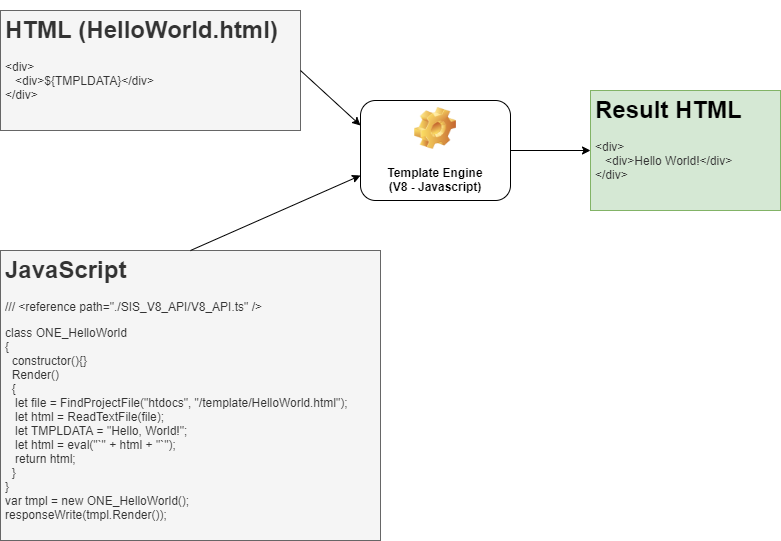
\includegraphics[width=1\textwidth]{template_engine}
	\caption{Funktionsweise Templating}
	\label{fig:template_engine}
\end{figure}

In dem gezeigten Beispiel \ref{fig:template_engine} kann man in HelloWorld.html \$\{TMPLDATA\} als Platzhalter erkennen. Dieser wird durch die 
Javascript Datei mit "Hello, World!" ersetzt. Links im Bild wird die resultierende HTML5 Datei gezeigt. 
Neue Agenten können sich dieser Mechanik bedienen, um individuelle Visualisierungen für die Clients zu erstellen.

\subsection{Digitales Handbuch für Integratoren als Nachschlagewerk}



\section{Wiederverwendbarkeit in spezifischeren C++-API-Agents}
